\section{Galaxias}

Todo sistema independiente de estrellas situado fuero de la Vía
Láctea, se le atribuye el nombre de galaxia. Las galaxias que poseen
un diámetro de entre 6.000 a 170.000 años luz, contienen entre 3.000
millones a 1 billón de estrellas, así como una cantidad de gas y polvo
que representa el 10\% de su masa total.

Las galaxias se clasifican, atendiendo a su morfología, en tres grandes
grupos:

\begin{enumerate}[a]
  \item Galaxias elípticas: Este conjunto de galaxias representan el
  20\% de las galaxias conocidas. Poseen forma esferoidal y carecen
  por completo de estructura interna definida. Además, no contienen
  apenas materia interestelar y las estrellas que la componen son
  viejas y se encuentran en estados muy avanzados de evolución.
  \item Galaxias espirales: Estas están divididas en dos grupos, el de
  las espirales normales y el de las espirales barradas. Las primeras,
  que representan el 75\% de todas las galaxias, tienen forma de lente
  aplanada y están dotadas de 2 a 3 brazos que parten de su centro,
  así como de gran cantidad de materia interestelar y muchas estrellas
  brillantes y jóvenes. La Vía Láctea pertenece este tipo. Por otro
  lado, las espirales barradas, disponen de dos brazos rectos opuestos
  que parten de su centro y de cuyos extremos surgen casi
  perpendicularmente sus brazos espirales, que en algunos casos se
  desarrollan hasta formar un círculo alrededor del núcleo.
  \item Galaxias irregulares: Representando el 5\% del total, su forma
  no presenta simetría alguna, siendo su aspecto y forma muy
  variables. Por lo general son pequeñas y contienen gran cantidad de
  materia interestelar. Se subdividen en las de tipo I, que pueden
  resolverse en estrellas, nebulosas o cúmulos, y las de tipo II, que
  no admiten este tipo de resolución y parecen ser completamente
  amorfas.
\end{enumerate}

\section{Apilado de imágenes. Aplicación post registro}

Las imágenes astronómicas obtenidas por cualquier telescopio se ven
limitadas por varios factores. Entre ellos, las condiciones
atmosféricas, la resolución del telescopio o la razón señal/ruido en
cada pixel de la imagen. La señal captada en cada pixel, depende del
flujo de la fuente astronómica o el tiempo de integración. El ruido
existente en cada pixel depende netamente del instrumento de
observación. Por ejemplo, en un circuito de carga acoplada (CCD), el
ruido se genera por la agitación térmica de los portadores de carga
(conductores), por la lectura del CCD y el ‘fondo’ de emisión del
cielo y/o telescopio. En general, un mayor tiempo de integración en
una fuente óptica proporciona imágenes con una señal mas expuesta al
ruido.

En la obtención de imágenes de radio el ruido se genera principalmente
por la agitación térmica de los receptores ubicados en cada
telescopio. Aquí, interacciones más largas dan lugar a imágenes con
mejores niveles de señal respecto al ruido, debido a que la
integración ya produce una disminución. Para un telescopio como ALMA,
la relación señal/ruido es inversamente proporcional a la raíz
cuadrada del producto del ancho de banda y el tiempo de integración
total. Es decir, para un ancho de banda fijo, la duplicación de la
señal al ruido requiere cuatro veces el tiempo de integración.

En el caso del observatorio ALMA, en muchos casos, no se detectan
objetos astronómicos individuales en una imagen, es decir, la señal de
éste objetivo es más pequeño que el ruido (o tres veces el ruido) en
la imagen. Sin embargo, si uno tiene una muestra de los objetivos (por
ejemplo, 1.000 fuentes) con posiciones conocidas con precisión, los
cuales están en la imagen, se podrían extraer sub-imágenes centradas
en cada posición y la media de todas las 1000 sub-imágenes. La imagen
promedio es equivalente a una imagen con 1000 veces el tiempo de
integración, es decir, el ruido en la imagen se reduce por un factor
de la raíz cuadrada de 1000 o aproximadamente 30. Por tanto, es más
probable que la imagen promediada muestre una detección de señales muy
débiles que requerirán de varios días o meses de observación (la
señal en la imagen promediada es la señal media de las 1000 fuentes,
mientras que el ruido es 30 veces menor que el ruido en cualquiera de
las imágenes en las 1000 fuentes). Ésta técnica, conocida como
apilamiento, es una herramienta muy potente y se utiliza por ejemplo,
en imágenes de rayos X, formación de imágenes ópticas e imágenes de
radio. El apilamiento da una idea de las características medias de una
muestra, algo muy útil para el análisis.

Como el archivo de ALMA sigue creciendo, una fracción cada vez mayor
del cielo está siendo capturada. Con una muestra suficientemente
amplia de objetos astronómicos, por ejemplo, un millón de cuásares con
posiciones precisas del Sloan Digital Sky Survey, SDSS, se encuentra
que muchos objetos de la muestra estarán en áreas que ya han sido
observadas por ALMA. Incluso, si no se detectan de forma individual,
se puede apilar todos los objetos que han sido vistos por ALMA y
obtener un flujo promedio para ésta muestra. Si la muestra también
tiene desplazamientos al rojo, el apilamiento se puede realizar en el
espacio de velocidades con el fin de obtener las propiedades medias de
cualquier línea de emisión dada.

\begin{figure}[hb!]
  \begin{center}
    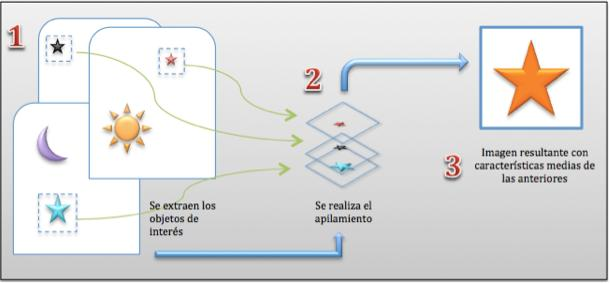
\includegraphics[scale=.5]{image/apilado}
  \end{center}
  \caption{Proceso de apilado de imágenes a partir de un conjunto de
  imágenes normalizadas.}
\end{figure}

\section{Inicios del apilado de imágenes}

Todas las observaciones de imágenes astronómicas poseen un umbral de
sensibilidad por debajo del cual los objetos no son detectables. Si
uno tiene razones para creer que en esa posición del cielo puede
existir algo, basándose en otras observaciones, se puede aplicar
apilamiento a una zona delimitada a un cierto rango de longitudes de
onda, pudiendo variar dicha longitud, y así conseguir el flujo medio
de emisiones.

En una aplicación inicial de esta técnica, Caillault y Helfand,
detectaron el flujo medio de rayos X de estrellas G en Pleiades,
utilizándola para determinar la edad respecto al deterioro de la
emisión. Los detectores de emisiones de rayos X han estado disponible
durante más de dos décadas, por lo que el apilamiento se ha convertido
en una técnica de análisis estándar. Las aplicaciones comenzaron desde
la determinación de la luminosidad media de rayos X, por ejemplo las
galaxias normales, galaxias Lyman y las fuentes de radio, para
determinar la emisión de rayos X de grupos distantes en el
Röntgensatellit (ROSAT) All-Sky Survey.

Los detectores digitales lineales han llegado a dominar los estudios
del cielo óptico e infrarrojo. La técnica de apilamiento ha sido
ampliamente adoptada: por ejemplo, Zibetti et al. detectaron la luz
intracluster apilando Sloan Digital Sky Estudio 683 (SDSS6); Lin et
al., apiló datos sobre las galaxias del cúmulo Two Micron All Sky
Survey (2MASS); Hogg et al. apiló datos del Keck IR para conseguir
galaxias de colores tenues; Minchin et al. fue tan lejos como para
apilar películas digitalizadas desde el telescopio Schmidt del Reino
Unido.